\documentclass[handout]{beamer}
%==============================================================
% Common Beamer Preamble for Course Lectures: Training and Scaling Language Models
%==============================================================

\usepackage[utf8]{inputenc}
\usepackage[T1]{fontenc}
\usepackage{hyperref}
\usepackage{amsmath,amssymb,xcolor,multicol,booktabs,colortbl}
\usepackage{graphicx,listings}
\renewcommand{\figurename}{Figure.}
\renewcommand{\tablename}{Table.}

% ---- TikZ Libraries ----
\usepackage{tikz}
\usetikzlibrary{positioning,arrows.meta,shapes.geometric,calc,fit,backgrounds,decorations.pathreplacing}

% ---- Presentation defaults ----
\setbeamertemplate{navigation symbols}{}
\setbeamersize{text margin left=0.55cm,text margin right=0.55cm}
\setbeamerfont{title}{size=\LARGE,series=\bfseries}
\setbeamerfont{subtitle}{size=\large}

% ---- FontAwesome fallback ----
\IfFileExists{fontawesome5.sty}{%
  \usepackage{fontawesome5}%
}{%
  \providecommand{\faMicrochip}{}%
  \providecommand{\faComments}{}%
  \providecommand{\faTools}{}%
  \providecommand{\faCheckCircle}{}%
  \providecommand{\faExclamationTriangle}{}%
  \providecommand{\faImage}{}%
  \providecommand{\faRobot}{}%
  \providecommand{\faTerminal}{}%
  \providecommand{\faBook}{}%
  \providecommand{\faRedo}{}%
  \providecommand{\faLayerGroup}{}%
  \providecommand{\faCogs}{}%
  \providecommand{\faDatabase}{}%
  \providecommand{\faHdd}{}%
  \providecommand{\faNetworkWired}{}%
}

% ---- Theme Style and Semantic Colors ----
%==============================================================
% Centralized Semantic Color Definitions for LLMs Presentation
%==============================================================

% ---- Base Template / Theme Colors (Aligned with Palette B) ----
\definecolor{themenavy}{RGB}{22,70,102}       % Palette B primary cerulean: #164666
\definecolor{themeblue}{RGB}{22,70,102}       % Primary alias
\definecolor{primarylight}{RGB}{34,92,132}    % Primary light: #225c84
\definecolor{themeteal}{RGB}{0,159,176}       % Accent cyan-teal: #009fb0
\colorlet{main_color}{themenavy}
\colorlet{accent}{themeteal}

\definecolor{accentdark}{RGB}{0,108,120}      % Deep cyan-teal for contrast text
\definecolor{accentlight}{RGB}{56,178,214}    % Slate accent cyan: #38b2d6
\definecolor{leafred}{RGB}{197,93,61}         % Terracotta red for branches/leaves

% ---- Website Panel & Border Neutrals ----
\definecolor{panelbg}{RGB}{237,245,249}       % Course-panel: #edf5f9
\definecolor{panelborder}{RGB}{204,226,238}   % Course-border: #cce2ee

% ---- Code listing style (syntax highlights) ----
\definecolor{deepblue}{RGB}{22,70,102}
\definecolor{deepred}{rgb}{0.6,0,0}
\definecolor{deepgreen}{RGB}{0,135,150}
\definecolor{halfgray}{gray}{0.55}

% ---- Semantic Theme Navy / Cerulean Shades ----
\colorlet{themebluebg}{panelbg}               % Panel #edf5f9
\colorlet{themebluecard}{main_color!8}        % Mild card background fills
\colorlet{themeblueborder}{panelborder}       % Border #cce2ee
\colorlet{themebluemid}{themeteal!60}         % Accent mid-contrast
\colorlet{themebluedraw}{main_color!80}       % Strong outline draws/strokes

% ---- Semantic Secondary Accent Teal Shades ----
\colorlet{accentdarkbg}{themeteal!10}        % Light secondary background fills
\colorlet{accentdarkdraw}{themeteal}         % Secondary outlines/strokes/text/axes

% ---- Functional Colors: Success Green ----
\definecolor{successgreen}{RGB}{55,145,55}
\colorlet{successbg}{successgreen!8}
\colorlet{successdraw}{successgreen!75}

% ---- Functional Colors: Alert Red ----
\definecolor{alertred}{RGB}{197,55,55}
\colorlet{alertbg}{alertred!8}
\colorlet{alertdraw}{alertred!75}

% ---- Functional Colors: Warning Orange ----
\definecolor{warningorange}{RGB}{220,110,30}
\colorlet{warningbg}{warningorange!10}
\colorlet{warningdraw}{warningorange!80}

% ---- Terracotta Red Shades ----
\colorlet{leafredbg}{leafred!12}
\colorlet{leafreddraw}{leafred!80}

% ---- Accent Violet (SWE-bench / observe phases) ----
\definecolor{accentviolet}{RGB}{120,70,180}
\colorlet{accentvioletbg}{accentviolet!10}
\colorlet{accentvioletdraw}{accentviolet!80}

% ---- Post-Training Axis Blue ----
\definecolor{posttrainingblue}{RGB}{40,90,165}
\colorlet{posttrainingbg}{posttrainingblue!8}
\colorlet{posttrainingdraw}{posttrainingblue!75}

% ---- Harness Component Action Green ----
\definecolor{actiongreen}{RGB}{55,145,55}
\colorlet{actiongreenbg}{actiongreen!10}
\colorlet{actiongreendraw}{actiongreen!65}

% ---- Harness Component Persist Olive ----
\definecolor{persistolive}{RGB}{120,135,40}
\colorlet{persistolivebg}{persistolive!12}
\colorlet{persistolivedraw}{persistolive!70}

% ---- Harness Component Observe Violet ----
\colorlet{observevioletbg}{accentvioletbg}
\colorlet{observevioletdraw}{accentvioletdraw}

% ---- Neutrals (Grays/Blacks) ----
\colorlet{neutralbg}{black!4}             % Very light background fills
\colorlet{neutrallight}{black!30}         % Border frames/ticks/dividers
\colorlet{neutraldark}{black!75}          % Main body text/code listing text

% ---- Beamer Block Color Overrides (Premium Terracotta Theme) ----
\setbeamercolor{block title alert}{bg=leafreddraw,fg=white}
\setbeamercolor{block body alert}{bg=leafredbg}
\setbeamercolor{alerted text}{fg=leafreddraw}

\usepackage{../common/style}
\graphicspath{{../common/figs/}{figs/}}

% ---- Code Listing Config ----
\lstset{
  basicstyle=\ttfamily\footnotesize,
  keywordstyle=\bfseries\color{deepblue},
  emphstyle=\ttfamily\color{deepred},
  stringstyle=\color{deepgreen},
  commentstyle=\color{halfgray}\itshape,
  numbers=left, numberstyle=\tiny\color{halfgray},
  backgroundcolor=\color{codebg},
  frame=l, framerule=1.5pt, rulecolor=\color{themeteal},
  xleftmargin=10pt, framexleftmargin=4pt, numbersep=6pt,
  showstringspaces=false, breaklines=true,
  aboveskip=4pt, belowskip=4pt
}

% ---- Image Placeholder Utility ----
\newcommand{\slideimage}[2][3.8cm]{%
  \begin{center}
    \begin{tikzpicture}
      \node[draw=main_color, dashed, very thick, rounded corners,
        fill=themebluebg, minimum width=0.88\linewidth, minimum height=#1,
      text width=0.80\linewidth, align=center, font=\itshape, text=accentdark]
      {\textbf{[ FIGURE / DIAGRAM ]}\\[6pt] #2};
    \end{tikzpicture}
  \end{center}
}

% ---- Concept Highlight Card Utility ----
\newcommand{\conceptcard}[3]{%
  \begin{coursebox}{#1}{#2}#3\end{coursebox}%
}

% ---- Reusable teaching-slide components ----
\newcommand{\learninggoals}[4]{%
  \begin{frame}{What should be clear by the end?}
    \begin{enumerate}
        \setlength{\itemsep}{7pt}
      \item #1
      \item #2
      \item #3
      \item #4
    \end{enumerate}
  \end{frame}
}

\newcommand{\checkpoint}[2]{%
  \begin{frame}{Checkpoint: #1}
    \begin{block}{Think, then compare}
      #2
    \end{block}
  \end{frame}
}

\newcommand{\takeaways}[4]{%
  \begin{frame}{The durable ideas}
    \begin{enumerate}
        \setlength{\itemsep}{8pt}
      \item #1
      \item #2
      \item #3
      \item #4
    \end{enumerate}
  \end{frame}
}

\newcommand{\smallsource}[1]{%
  \vfill\hfill{\tiny\color{neutraldark}Source: #1}
}

% ---- Logo on content frames ----
\newif\ifplacelogo
\placelogotrue
\logo{\ifplacelogo
  \raisebox{-0.3ex}{
\includegraphics[height=0.4cm]{IMT_Atlantique_logo.png}}%
\fi}

\makeatletter
\define@key{beamerframe}{nologo}[true]{%
  \placelogofalse
}
\makeatother

% Fix Beamer bold font warning: substitute undefined T1/cmss/b/n with T1/cmss/bx/n
\DeclareFontShape{T1}{cmss}{b}{n}{<->ssub * cmss/bx/n}{}

% Default Author & Institute metadata
\author[Jonathan Lys]{Jonathan Lys}
\institute[IMT Atlantique]{IMT Atlantique}

% ---- Front Page / Title Slide Macro ----
% Displays Title + IMT Atlantique logo and Brain logo
\newcommand{\makelecturetitle}[1][Training and Scaling Language Models: From First Principles to Efficient Serving]{%
  \placelogofalse
  {
    \setbeamertemplate{footline}{}
    \settitletagline{#1}
    \settitlelogos{%
      \raisebox{-0.5\height}{
\includegraphics[height=1.15cm]{IMT_Atlantique_logo.png}}%
      \hspace{1.2em}%
      \raisebox{-0.5\height}{\includegraphics[height=1.15cm]{brain.pdf}}}
    \begin{frame}[plain]
      \titlepage
    \end{frame}
  }
  \placelogotrue
}

% Section TOC Frame
\AtBeginSection[]{\coursesectiondivider}

\title[TLM -- Session 10]{Session 10: Context and Pipeline Parallelism\\[4pt]
\normalsize\itshape Splitting Sequence Length and Model Depth}
\date{\today}

\begin{document}
\makelecturetitle
\begin{frame}{Lecture map}
  \tableofcontents
  \vfill
  \begin{block}{Guiding question}
    When width sharding is not enough, how do we divide long contexts and deep models without losing exactness or utilization?
  \end{block}
\end{frame}
\learninggoals
  {Distinguish context parallelism from sequence parallelism.}
  {Explain exact ring attention through online softmax.}
  {Compute pipeline bubbles for a micro-batch schedule.}
  {Map parallel dimensions to a real cluster topology.}

\section{Context parallelism}

\begin{frame}{Two techniques shard the sequence axis for different reasons}
  \begin{columns}[t]
    \begin{column}{0.47\linewidth}
      \begin{block}{Sequence parallelism}
        Complements tensor parallelism by sharding token activations around norms, dropout, and elementwise operations.
      \end{block}
    \end{column}
    \begin{column}{0.47\linewidth}
      \begin{block}{Context parallelism}
        Splits a long context across devices so each rank stores only part of the queries and token activations.
      \end{block}
    \end{column}
  \end{columns}
  \begin{alertblock}{The hard part}
    Attention couples every local query with keys and values that may live on every other rank.
  \end{alertblock}
\end{frame}

\begin{frame}{Most layers are local after token sharding}
  With $T$ split over $C$ context ranks, each rank owns roughly $T/C$ positions.
  \begin{itemize}
    \setlength{\itemsep}{7pt}
    \item tokenwise normalization and MLPs operate locally
    \item residual additions operate locally
    \item attention needs remote key-value blocks
    \item some losses and metrics need global reductions
  \end{itemize}
  \begin{block}{Memory effect}
    Token activation memory falls roughly with $1/C$, while communication appears inside every attention layer.
  \end{block}
\end{frame}

\begin{frame}{Ring attention rotates key-value blocks}
  \centering
  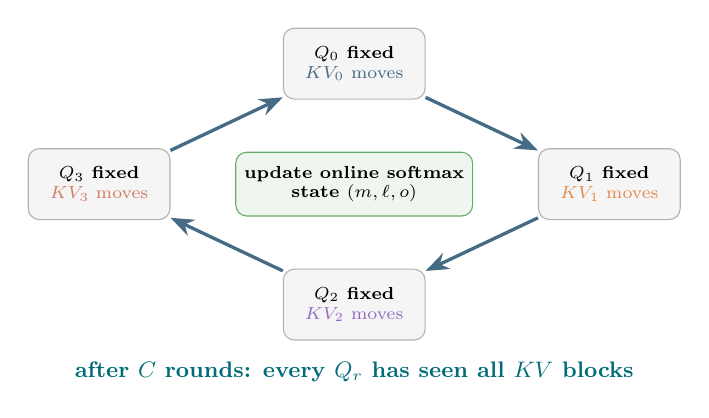
\begin{tikzpicture}[x=1cm,y=1cm,scale=.9,transform shape,every node/.style={font=\scriptsize},
    rank/.style={draw=neutrallight,fill=neutralbg,rounded corners,minimum width=2.0cm,minimum height=1.0cm,align=center}]
    \node[rank] (r0) at (5.4,3.7) {\textbf{$Q_0$ fixed}\\\color{themebluedraw}$KV_0$ moves};
    \node[rank] (r1) at (9.0,2.0) {\textbf{$Q_1$ fixed}\\\color{warningdraw}$KV_1$ moves};
    \node[rank] (r2) at (5.4,.3) {\textbf{$Q_2$ fixed}\\\color{accentvioletdraw}$KV_2$ moves};
    \node[rank] (r3) at (1.8,2.0) {\textbf{$Q_3$ fixed}\\\color{leafreddraw}$KV_3$ moves};
    \draw[-{Stealth},very thick,themebluedraw] (r0)--(r1);
    \draw[-{Stealth},very thick,themebluedraw] (r1)--(r2);
    \draw[-{Stealth},very thick,themebluedraw] (r2)--(r3);
    \draw[-{Stealth},very thick,themebluedraw] (r3)--(r0);
    \node[draw=successdraw,fill=successbg,rounded corners,align=center,minimum width=3.1cm,minimum height=.9cm,font=\scriptsize\bfseries] at (5.4,2.0) {update online softmax\\state $(m,\ell,o)$};
    \node[text=accentdark,font=\small\bfseries] at (5.4,-.65) {after $C$ rounds: every $Q_r$ has seen all $KV$ blocks};
  \end{tikzpicture}
  \begin{alertblock}{Memory behavior}
    Only a few $KV$ blocks are resident per rank; no rank gathers the full context or materializes a global $T\times T$ score matrix.
  \end{alertblock}
  \smallsource{Hugging Face Ultra-Scale Playbook and Ring Attention}
\end{frame}

\begin{frame}{Online softmax makes blockwise attention exact}
  For one query row, maintain running maximum $m$, normalizer $\ell$, and numerator $o$.
  For a new score block with maximum $m_b$:
  \[
    m'=\max(m,m_b)
  \]
  \[
    \ell'=e^{m-m'}\ell+\sum_j e^{s_j-m'}
  \]
  \[
    o'=e^{m-m'}o+\sum_j e^{s_j-m'}v_j
  \]
  Final attention is $o/\ell$. Rescaling preserves contributions computed under earlier maxima.
\end{frame}

\begin{frame}{Causal attention can imbalance ring work}
  Early query positions have few valid keys. Late queries have many. A naive contiguous partition gives ranks unequal useful work after masking.
  \begin{columns}[t]
    \begin{column}{0.47\linewidth}
      \begin{alertblock}{Symptom}
        Some ranks wait while others process large valid attention regions.
      \end{alertblock}
    \end{column}
    \begin{column}{0.47\linewidth}
      \begin{block}{Mitigation}
        Interleave or pair early and late context blocks so valid attention work is balanced.
      \end{block}
    \end{column}
  \end{columns}
\end{frame}

\section{Pipeline parallelism}

\begin{frame}{Pipeline parallelism assigns layer ranges to stages}
  \begin{center}
  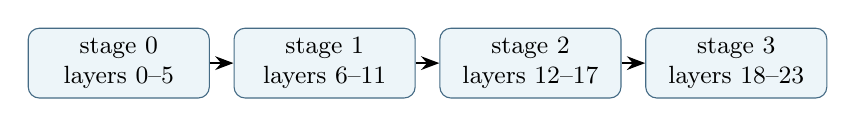
\begin{tikzpicture}[node distance=.30cm,every node/.style={font=\small},box/.style={draw=themebluedraw,fill=themebluebg,rounded corners,align=center,minimum width=2.3cm,minimum height=.7cm}]
    \node[box] (s0) {stage 0\\ layers 0--5};
    \node[box,right=of s0] (s1) {stage 1\\ layers 6--11};
    \node[box,right=of s1] (s2) {stage 2\\ layers 12--17};
    \node[box,right=of s2] (s3) {stage 3\\ layers 18--23};
    \draw[-{Stealth},thick] (s0)--(s1);
    \draw[-{Stealth},thick] (s1)--(s2);
    \draw[-{Stealth},thick] (s2)--(s3);
  \end{tikzpicture}
  \end{center}
  \begin{block}{Why micro-batches?}
    Split a global batch into $M$ micro-batches so different stages can work on different micro-batches concurrently.
  \end{block}
\end{frame}

\begin{frame}{Pipeline bubbles shrink as micro-batches increase}
  For $P$ balanced stages and $M$ forward-only micro-batches:
  \[
    \text{ideal utilization}\approx\frac{M}{M+P-1}
  \]
  \begin{block}{Worked example}
    $P=4$, $M=8$ gives $8/(8+3)\approx73\%$ idealized forward utilization. With $M=32$, it rises to about $91\%$.
  \end{block}
  \begin{alertblock}{Trade-off}
    More micro-batches reduce bubbles but can create smaller, less efficient kernels and more activation bookkeeping.
  \end{alertblock}
\end{frame}

\begin{frame}{AFAB and 1F1B trade memory for schedule complexity}
  \begin{columns}[t]
    \begin{column}{0.47\linewidth}
      \begin{block}{All-forward-all-backward}
        simple schedule\\many outstanding activations\\higher peak memory
      \end{block}
    \end{column}
    \begin{column}{0.47\linewidth}
      \begin{block}{One-forward-one-backward}
        after warmup, alternate directions\\fewer stored activations\\more coordination
      \end{block}
    \end{column}
  \end{columns}
  \vfill
  Both still have warmup and cooldown bubbles. Interleaving virtual stages can reduce them further at added complexity.
\end{frame}

\begin{frame}{The slowest stage sets pipeline throughput}
  \[
    t_{\text{cycle}}\approx\max_s t_s
  \]
  \begin{itemize}
    \setlength{\itemsep}{7pt}
    \item Equal layer counts need not mean equal work.
    \item Embeddings, output projection, and activation sizes can skew stages.
    \item Stage boundaries determine activation communication volume.
    \item Profile stage time and memory before moving boundaries.
  \end{itemize}
\end{frame}

\checkpoint{schedule arithmetic}
  {For six stages and twelve micro-batches, estimate idealized forward utilization. Name two real effects that make measured utilization lower.}

\section{Composing parallel dimensions}

\begin{frame}{The device count factorizes across parallel groups}
  \[
    N_{\text{GPU}}=D\times T_p\times C\times P
  \]
  \small
  \begin{tabular}{lll}
    \toprule
    Dimension & Splits & Communication pattern \\
    \midrule
    data / FSDP & batch and model state & gradient or shard collectives \\
    tensor & hidden width and heads & frequent activation collectives \\
    context & sequence positions & key-value exchange per layer \\
    pipeline & layer depth & point-to-point activations \\
    \bottomrule
  \end{tabular}
\end{frame}

\begin{frame}{Map the chattiest group to the fastest fabric}
  \begin{enumerate}
    \setlength{\itemsep}{7pt}
    \item Use tensor parallelism inside a high-bandwidth GPU island.
    \item Add context parallelism when token activations or attention exceed local memory.
    \item Use pipeline parallelism when model depth spans nodes.
    \item Replicate the resulting model group with data parallelism when batch and devices remain.
  \end{enumerate}
  \begin{alertblock}{Selection rule}
    Choose the smallest degree on each axis that resolves a concrete memory or compute constraint.
  \end{alertblock}
\end{frame}

\begin{frame}{Four cases lead to different strategies}
  \small
  \begin{tabular}{p{.41\linewidth}p{.49\linewidth}}
    \toprule
    Binding constraint & First strategy to evaluate \\
    \midrule
    model fits, short context, more GPUs & DDP or FSDP replicas \\
    one wide layer does not fit & tensor parallelism \\
    weights fit, 128k-token examples do not & context parallelism plus checkpointing \\
    model exceeds one node & pipeline across nodes, TP within node \\
    \bottomrule
  \end{tabular}
\end{frame}

\checkpoint{cluster design}
  {Design a layout for 32 GPUs arranged as four 8-GPU nodes. State the memory constraint, proposed $D,T_p,C,P$, and which communication crosses node boundaries.}

\takeaways
  {Context parallelism shards tokens and uses exact blockwise attention with online softmax.}
  {Pipeline parallelism shards depth, while micro-batches trade bubble size against memory and kernel efficiency.}
  {Load balance matters across causal context blocks and pipeline stages.}
  {Parallel dimensions should follow the workload constraint and physical network hierarchy.}
\end{document}
